На рисунке \ref{fig:funcmodel} представлены результаты функционального моделирования. На временной диаграмме продемонстрирована нормальная работа устройства: включение, работа, чтение режима, выключение, включение с другим адресом и т.д. Продемонстрированы разные режимы работы и переключения между ними.
\begin{figure}
  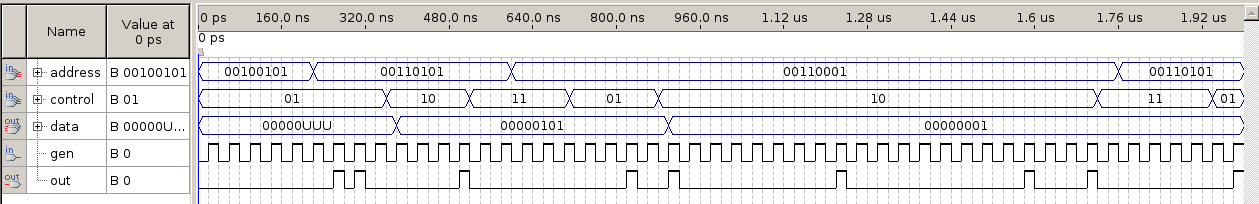
\includegraphics[scale=0.5]{./func-switching.png}
  \caption{Функциональное моделирование узла.}
  \label{fig:funcmodel}
\end{figure}